\documentclass[9pt]{article}

% Language setting
% Replace `english' with e.g. `spanish' to change the document language
\usepackage[english]{babel}

% Set page size and margins
% Replace `letterpaper' with`a4paper' for UK/EU standard size
\usepackage[a4paper,top=2cm,bottom=2cm,left=3cm,right=3cm,marginparwidth=1.75cm]{geometry}

% Useful packages
\usepackage{amsmath}
\usepackage{tikz}
\usepackage{graphicx}
\usepackage{mwe}
\usepackage{fullpage}
\usepackage{hyperref}
\hypersetup{linkcolor=blue, urlcolor=blue, colorlinks}
\usepackage{caption}
\usepackage{subcaption}
\usepackage{float}

\title{Assignment 2: \\ Programming in CUDA \\ \large \textit{Accelerator-based Programming}}
\author{Oskar Tegby}
\date{October 2022}

\setlength{\parindent}{0pt}

\begin{document}
\maketitle

\begin{tikzpicture}[remember picture, overlay]
  \node [anchor=north west, inner sep=25pt]  at (current page.north west)
     {
\includegraphics[height=3.3cm]{uu_logo.png}};
\end{tikzpicture}

\section{Introduction}
This assignment studies the computational properties of \texttt{CUDA} implementations of matrix-vector and matrix-matrix multiplication. The former is parallelized only over the rows, and the latter over both rows and columns, which is assumed to be faster than only parallelizing over the rows in the latter case. Notably, these operations are completely parallelizable since they are fully data parallel. Thus, we will dedicate this report almost exclusively to reporting and discussing the achieved bandwidth of the different implementations. Lastly, all tests are run on a \texttt{Nvidia Tesla T4} graphics card running on the \texttt{Snowy} server on the \texttt{UPPMAX} cluster. \\

The veracity of the code is tested by comparing the results for a matrix, A, and a vector, x, with strictly increasing values, since that is fully asymmetric. That is, we tested the code with e.g.
\begin{align*}
    A=
    \begin{bmatrix}
        1 & 2 & 3 & 4 \\
        5 & 6 & 7 & 8 \\
        9 & 10 & 11 & 12 \\
        13 & 14 & 15 & 16 \\
    \end{bmatrix}
    \quad\text{and}\quad
    x=
    \begin{bmatrix}
        1 \\
        2 \\
        3 \\
        4
    \end{bmatrix},
\end{align*}
as input values, which gives us the output
\begin{align*}
    b=
    \begin{bmatrix}
        30 & 70 & 110 & 150
    \end{bmatrix}.
\end{align*}
This indicates that the implementation is indeed correct. \\

Furthermore, all results are computed as the averages of 20 tests each run with 20 repeats to decrease the influence of computational noise, which allows us to rely on smaller details in the obtained graphs. Thus, it should not be seen as an explanation for unexpected behavior, as is commonly the case. 
\section{Tasks}
\subsection{Task 1}
\subsubsection{Part A}
Figure \ref{fig:mv_native_mult} shows the throughput of the single-precision matrix-vector multiplication run with N = M ranging from 104 to 9576 obtained by running the code with \texttt{block\_size} = 512. The throughput is computed as
\begin{align*}
    (MN + N + M)\cdot\texttt{sizeof}(\texttt{float})\cdot 10^{-9}/t_{\text{best}}.
\end{align*}
\subsubsection{Part B}
Figure \ref{fig:native_loglog} shows a linear increase in throughput with the tensor sizes until about $N=M=3000$. Afterwards, the throughput stagnates between above 200 and 240 GB/s. The reason for which is that we can no longer fit the entire matrix in our local cache, which means that we have to fetch the data from the graphics memory, which has a bandwidth of 320 GB/s on the Nvidia T4 graphics card. This constitutes a theoretical upper bound which we should not expect to reach. \\

However, we should neither expect to miss out on 80 GB/s throughput with such ideal parallelism. Given that the code is coalesced, since each thread runs the \texttt{for} loop with jumps of size $N$, this comes as a surprise and is a mystery to the author. Here, we must recall that we have implemented a column-major matrix layout, which means that every column is contiguously stored in memory, and each row requires a jump of size $N$ to reach the next element. Hence, instead of the first thread accessing memory loading the first row, and the other threads using the other elements of that row, the same happens but for columns instead of rows. This causes the implementation to look uncoalesced at a first glance. \\

The choice of the block size 128 comes from each warp being 32 threads large and the fact that they are running on the same streaming multiprocessor (SM): We want to run several warps on each SM since we have to keep the it busy. That is, if the threads in one warp need to wait for data, then they can be swapped out to another warp which has fetched its data. At the same time, we want to make sure that the work is distributed among all SMs, so we do not want to run too many warps on each SM. However, since the maximum block size is 1028, this would only amount to 32 warps, which is a lot less than the amount of available parallel work. \\

The choice of the grid size as 
\begin{align*}
	\texttt{n\_blocks}=(N \cdot M +\texttt{block\_size} - 1) / \texttt{block\_size}
\end{align*}
comes from dividing the number of elements from the matrix by the chosen \texttt{block\_size}, and rounding up by adding $\texttt{block\_size} - 1$ in the numerator. This splits up the work into \texttt{n\_blocks} blocks of work, each with a block size of \texttt{block\_size}. Thus, we have \texttt{n\_blocks} blocks done in parallel, and each of those are worked on in parallel since we split the block size into warps, which are run in parallel on each SM. \\

From these settings we expect a speedup of $\texttt{n\_blocks}$ as that is the number of blocks computed in parallel. However, the throughput that we get is limited by the bandwidth and latency of the device's memory hierarchy, as well as the memory properties of the implementation of the kernel, as discussed in the second paragraph of this subsection.
\begin{figure}[!ht]
    \centering
    \begin{subfigure}[b]{0.49\textwidth}
        \centering
        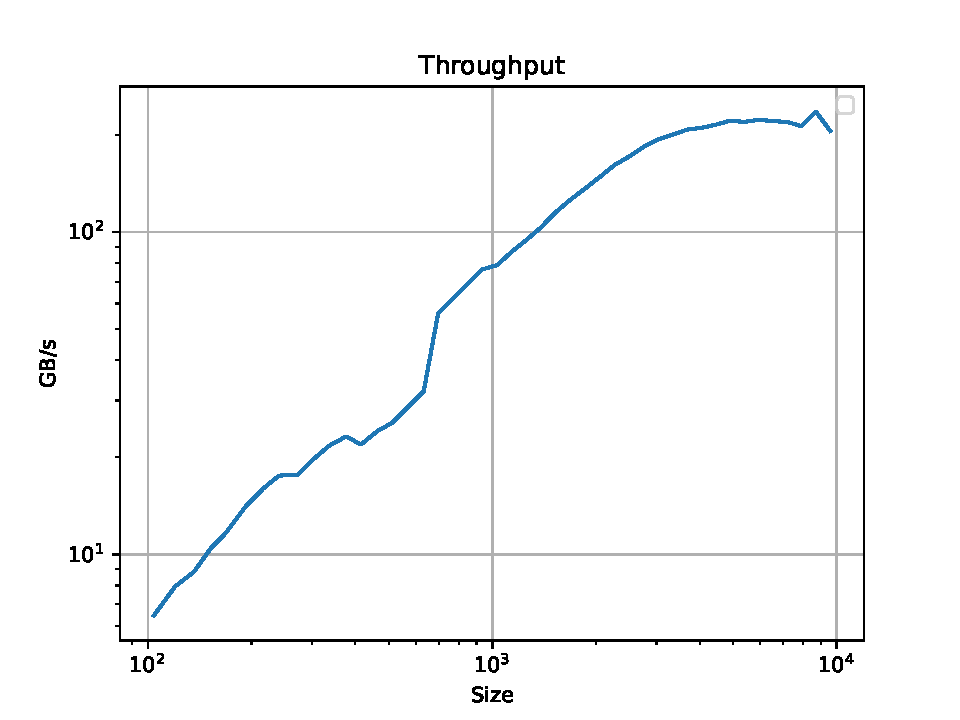
\includegraphics[width=\linewidth]{figs/loglog.pdf}
        \caption{The increase with loglog scale.}
        \label{fig:native_loglog}
    \end{subfigure}\hfill
    \begin{subfigure}[b]{0.49\textwidth}
        \centering
        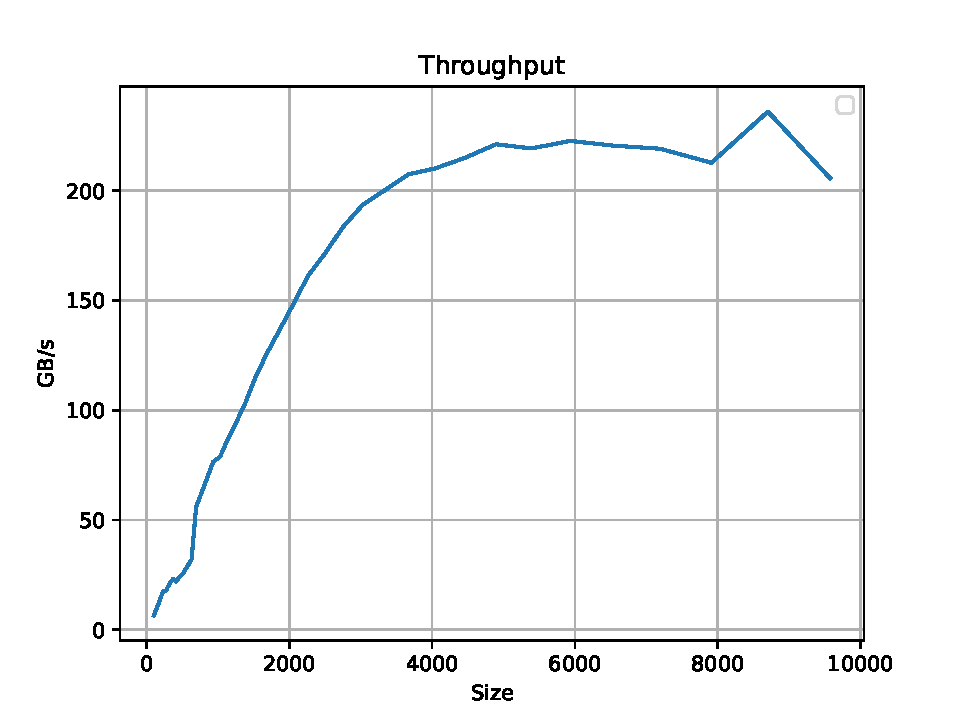
\includegraphics[width=\linewidth]{figs/linear.pdf}
	\caption{The increase with linear scale.}
	\label{fig:native_linear}
    \end{subfigure}\hfill
    \caption{Native matrix-vector multiplication with $M=N$ ranging from 100 to 10000.}
    \label{fig:mv_native_mult}
\end{figure}
\subsection{Task 2}
\subsubsection{Part A}
The results using cuBLAS are found in Figure \ref{fig:mv_cublas_mult}. There, we observe roughly the same behavior as in Figure \ref{fig:mv_native_mult}, aside from a much steeper increase in throughput and one occuring for much smaller problem sizes. That is presumably because cuBLAS is optimized for those scenarios than what any elementary native implementation could be. Furthermore, as expected, the peak throughput is also higher in this scenario. However, it is, notably, 70 GB/s short of the theoretical maximum, which still must be considered quite low given that it is only 80\% of what the bandwidht allows. Importantly, this supports the notion that it was not an error in the memory coalescing that caused the relatively slow native implementation. The reason for these behaviors still remains unknown. 
\begin{figure}[!ht]
    \centering
    \begin{subfigure}[b]{0.49\textwidth}
        \centering
        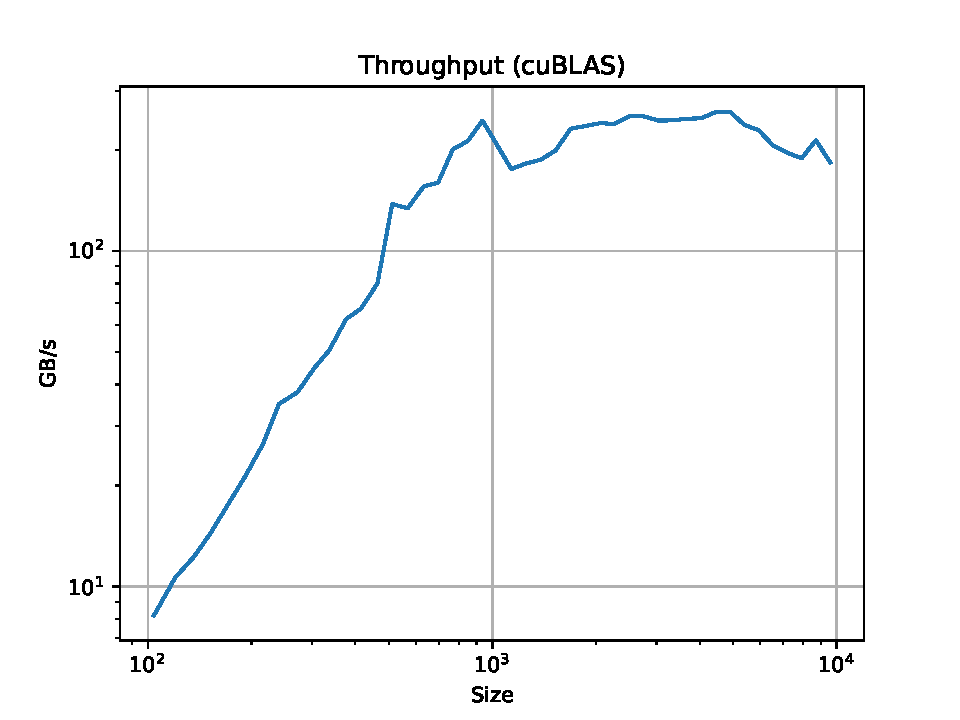
\includegraphics[width=\linewidth]{figs/cublas_loglog.pdf}
        \caption{The increase with loglog scale.}
        \label{fig:cublas_loglog}
    \end{subfigure}\hfill
    \begin{subfigure}[b]{0.49\textwidth}
        \centering
        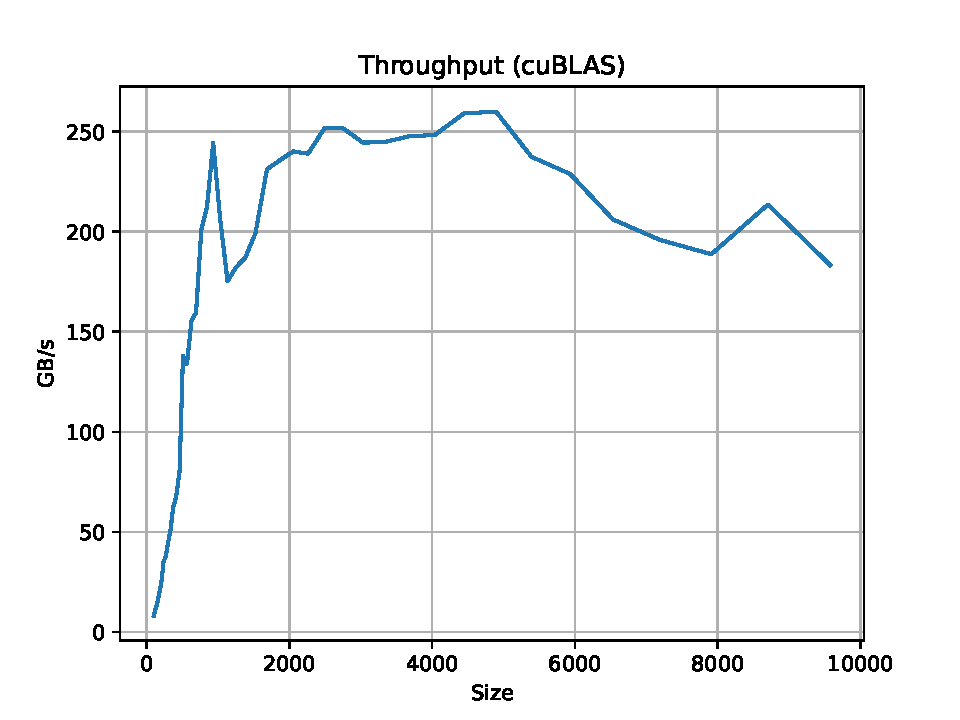
\includegraphics[width=\linewidth]{figs/cublas_linear.pdf}
	\caption{The increase with linear scale.}
	\label{fig:cublas_linear}
    \end{subfigure}\hfill
    \caption{cuBLAS matrix-vector multiplication with $M=N$ ranging from 100 to 10000.}
    \label{fig:mv_cublas_mult}
\end{figure}
\subsubsection{Part B}

\subsubsection{Part C}
\subsection{Task 3}
\subsection{Task 4}
\end{document}
\subsubsection{Part B}
\subsubsection{Part C}
\subsection{Task 3}
\subsection{Task 4}
\end{document}
